\chapter{Thực nghiệm và đánh giá}
\thispagestyle{fancy}

\section{Thực nghiệm}

\subsection{Xữ lí dữ liệu}

\begin{itemize}
    \item Dữ liệu được thu thập từ 44 người với những độ tuổi và giới tính khác nhau, kèm theo đó là những ghi chú về nhịp tim của bệnh nhân, trong đó một số dữ liệu không được sử dụng: 102, 104, 107, 217 do những bệnh nhân này có sử dụng máy trợ tim (peatmaker) nên nhịp tim không tự nhiên ảnh hưởng đến quá trình phân loại.
    \item Dữ liệu trong thử nghiệm được lấy trên chuyển đạo Lead II trong 2 channel của dữ liệu MIT-BIH (channel 1) vì chuyển đạo này thể hiện rõ ràng nhất đặc điểm của ECG.
    \item Dữ liệu được thu thập với tốc độ lấy mẫu là 360 mẫu/s. Một bản ghi từ một bệnh nhân được ghi lại trong khoảng 30 phút. Một bản ghi có 650 000 mẫu. Sau khi trích xuất đặc trưng khoảng R-R và chuẩn hóa về cùng hình dạng thì mỗi khoảng R-R có độ dài là 324.
    \item Dữ liệu sau khi qua giai đoạn lọc nhiễu và cắt đoạn RR thu được 108724 mẫu tín hiệu bao gồm (74546 bình thường và 29178 bất thường).
\end{itemize}
\begin{center}
    \begin{tabular}{|c|c|}
    \hline 
    Tập dữ liệu huấn luyện & Tập dữ liệu kiểm thử \\ 
    \hline 
    81149 & 22399\\
    \hline 
    \end{tabular}
\end{center}

\subsection{Kết quả}
Kết quả được đánh giá theo độ đo: Precision, Recall, F1-score, Accuracy, Loss.
\begin{center}
    \begin{tabular}{|c|c|c|}
    \hline
    Estimate & Normal & Abnormal\\
    \hline 
    Precision & 0.96 & 0.74\\ 
    \hline 
    Recall & 0.87 & 0.92\\
    \hline 
    F1-score & 0.90 & 0.81\\
    \hline 
    Accuracy & \multicolumn{2}{|c|}{0.95} \\
    \hline 
    Loss & \multicolumn{2}{|c|}{0.03} \\
    \hline
    \end{tabular}
\end{center}
\begin{center}
    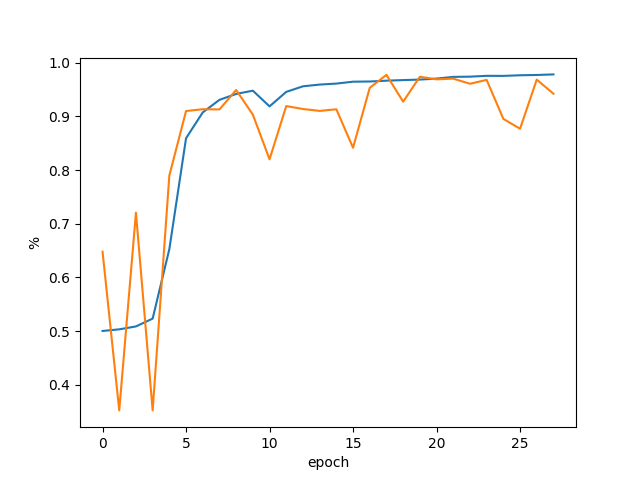
\includegraphics[scale=.6]{image/chapter6/acc.png}
    \begin{figure}[htp]
    \begin{center}
    \end{center}
    \caption{Độ chính xác của quá trình huấn luyện và kiểm thử}
    \end{figure}
\end{center}
\begin{center}
    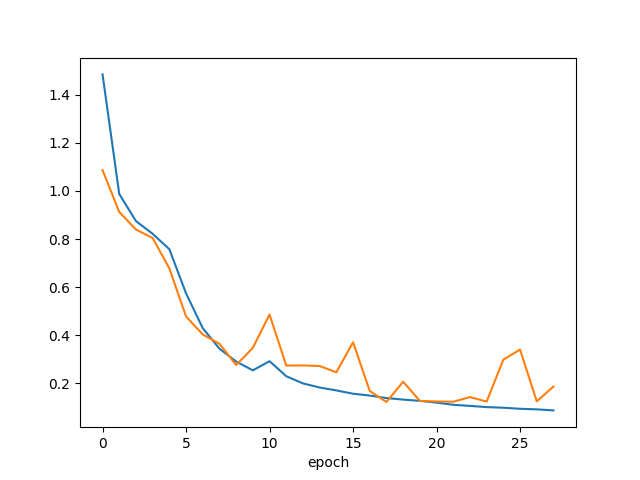
\includegraphics[scale=.6]{image/chapter6/loss.png}
    \begin{figure}[htp]
    \begin{center}
    \end{center}
    \caption{Độ mất mát của quá trình huấn luyện và kiểm thử}
    \end{figure}
\end{center}

\subsection{Đánh giá}
\begin{itemize}
    \item Độ chính xác của mô hình phân loại chưa được cao như những nghiên cứu khác.
\end{itemize}
\subsection{Trở ngoại}
\begin{itemize}
    \item Chỉ mới áp dụng mô hình phân loại trên chuyển đạo Lead II.
    \item Những vấn đề trong việc xử lý dữ liệu, nhiễu...
\end{itemize}
